% !TEX root = ../notes_3dprinting.tex
% Chapter 11: Printing TPU -- WRITTEN
% The hands-on feed/print/unfeed procedure for TPU on the external spool
% holder. Chapter 6 (Materials) covers why TPU cannot go through the AMS;
% this chapter covers what to actually do about it at the machine.
%%%%%%%%%%%%%%%%%%%%%%%%%%%%%%%%%%%%%%%%%%%%%%%%%%%%%%%%%%%%%%%%%%%%%%

\index{TPU}\index{external spool}
\chapter{TPU}\label{ch:tpu}
\printchapterversion{11_tpu}
\newthought{Load It, Print It, Load It Back.}

\marginnote{{\centering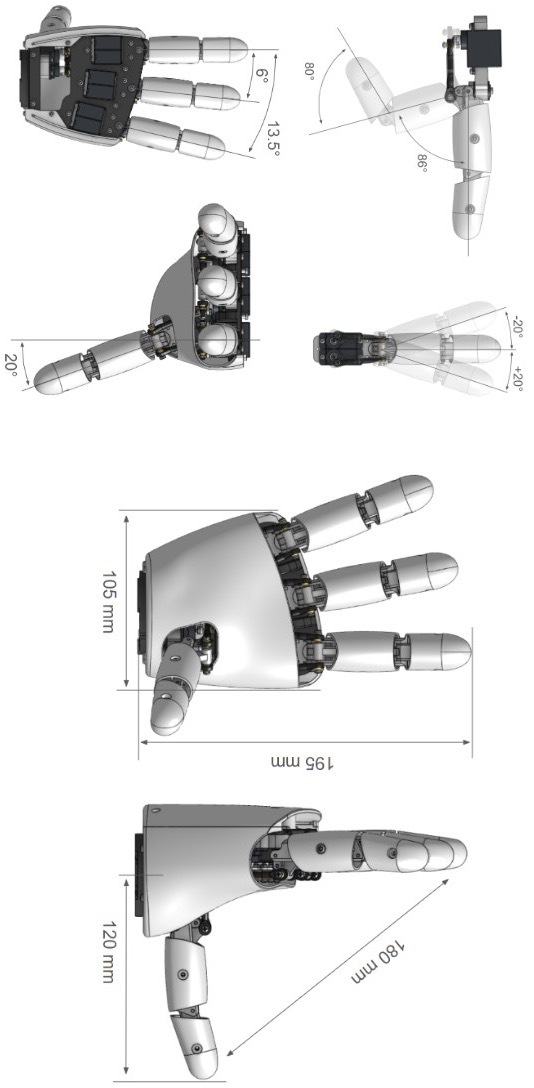
\includegraphics[width=0.75\marginparwidth]{figures/amazinghand.jpg}\par}
\newthought{Why TPU?} It is strong yet stays flexible after
printing. We first used it for a robotic skin on the AmazingHand by
Pollen Robotics, pictured above, making a gripper surface more adaptable
and raising grip success rates.}

\index{AMS}\newthought{TPU runs from the external spool holder.} TPU never goes through the AMS. The flexible filament coils
inside the AMS hub instead of advancing down its Bowden path. You don't want to spend the time cleaning this.
So this is a mishap to avoid and not to experience first-hand for a deeper learning experience. 
Because we can not use the AMS, we have to feed TPU directly into the extruder. 
This is a hands-on procedure that requires some care and attention.

\index{unloading filament}\newthought{unloading pla}
\begin{enumerate}[itemsep=2pt]
  \item On the printer screen open the gear \icongear{}, then
        \texttt{Filament}, and unload whatever is currently sitting in the
        extruder.
  \item Detach the tube on the back that runs from the AMS into the toolhead and
        park it clear of the feed path.
\end{enumerate}

\index{loading filament}\newthought{loading tpu}
\begin{enumerate}[itemsep=2pt]
  \item Hang the TPU spool on the external holder at the back of the
        printer (looks like a metal bar) and thread the loose end into the
        tube inlet the AMS tube used to occupy.
  \item On the printer screen choose the nozzle \iconnozzle{} icon, then
        \texttt{Feeding}, choose \texttt{Load}. While the printer runs the load, push the
        filament slightly in by hand until the feed gears grab it and
        take over. Watch the nozzle purge until a clean strand of TPU comes out. 
  \item In Bambu Studio open the \texttt{Device} tab. Next to the four
        AMS slots sits an \texttt{Ext} slot\index{Ext slot} for the external spool; select
        that one and set the filament type to \texttt{TPU}. 
\end{enumerate}


\marginnote{\newthought{One object per plate for a nicer result.} TPU's elasticity stretches into a hair
that drifts and tangles with movement between objects while printing. This messes up your surface and print quality.}

\index{stringing}\newthought{You are ready to print TPU.}  

\index{drying}\newthought{unloading tpu}
\marginnote{\newthought{Keep the spool dry.} TPU is hygroscopic. Off the
holder, store the spool in a sealed box with desiccant. A spool left in
open room air for a few days prints visibly worse.}
\begin{enumerate}[itemsep=2pt]
  \item On the printer screen choose the nozzle \iconnozzle{} icon, then
        \texttt{Feeding}, choose \texttt{Unload}. The printer heats the
        nozzle and retracts the filament.
  \item Once the feed gears release it,
  pull the strand back out of the tube inlet by hand and wind it
  onto the spool. Stow away TPU in a sealed box immediately.
\end{enumerate}

\newthought{loading pla again}
\begin{enumerate}[itemsep=2pt]
  \item Reattach the AMS tube you parked earlier to the tube inlet on the
        toolhead and push it in until it seats.
  \item On the printer screen open the gear \icongear{}, then
        \texttt{Filament}, select the AMS slot holding your PLA, and
        choose \texttt{Load}. The AMS feeds the filament down the Bowden
        path on its own; watch the nozzle purge until a clean strand of
        PLA comes out.
  \item In Bambu Studio open the \texttt{Device} tab and select the AMS
        slot instead of the \texttt{Ext} slot, so the next job pulls from
        the AMS again.
\end{enumerate}





